\section{연구 방법 및 과정}

<<<<<<< HEAD
\subsection{데이터 파악}

해양위성센터에서 제공하는 SST 데이터를 다운받을 수 있는 경로를 확인하였다. 접근할 수 있는 데이터는 2020년 4월 29일 기준으로 Table \ref{table:KOSC-SST-data}\와 같다.


\begin{table}[!htbp]
	\caption{해양위성센터에서 다운로드 가능한 SST 데이터.}
	\begin{tabular}{c|c|c}
		\toprule
		센서명           & 자료시작시기       & 자료종료시기 (2020. 4. 29. 기준) \\ \toprule
		AVHRR         & 2011. 9. 1.  & 2020. 4. 21.          \\ \hline
		MODIS (Aqua)  & 2011. 9. 1.  & 2020. 4. 6.           \\ \hline
		MODIS (Terra) & 2011. 9. 1.  & 2020. 4. 7.           \\ \hline
		VIIRS         & 2016. 6. 17. & 2020. 4. 27.          \\ \bottomrule
	\end{tabular}

	\label{table:KOSC-SST-data}
\end{table}

NOAA/AVHRR 자료는 Fig. \ref{fig:asc_file}\와 같이 텍스트 파일의 형태로 배포되고 있다는 것을 알 수 있었다. 총 4개의 열로 저장되어 있으며, 첫번째 열부터 각각 인덱스, 위도, 경도, SST 임을 알 수 있는데, 자료가 산출되지 않은 경우에 ***로 표시되어 있다.

\begin{figure}[htbp]
	\centerline{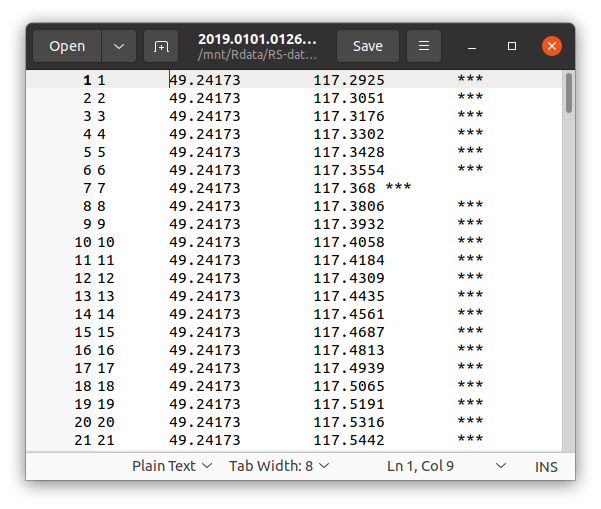
\includegraphics[width=12cm]{asc_file1}}
	\caption{NOAA/AVHRR SST 자료 텍스트 파일 캡처 화면.}
	\label{fig:asc_file}
\end{figure}

Terra/Aqua 위성의 MODIS를 구한 SST 자료는 HDF(Hierarchical Data Format) 형태로 배포되었다. HDF는 이름 그대로 계층적으로 구조화된 다차원 배열 데이터를 저장하기 위하여 HDF Gruop(https://www.hdfgroup.org/)에 의해 만들어진 파일 형식이다.

\newpage
\subsection{연구에 사용한 데이터}

해양위성센터에서 배포한 MODIS의 SST 데이터는 구름이 제거되지 않아서 SST 값에 심각한 오류를 포함하고 있어 사용하지 않고, NOAA/AVHRR의 SST 레벨2 자료를 이용하여 연구를 진행하였다. 

NOAA/AVHRR의 SST 레벨2 자료는 앞서 언급한 것 처럼 텍스트 파일 형태로 제공되고 있고, Figure \ref{fig:SST-KOSC}\와 같이 지도 위에 표출된 자료도 함께 제공되고 있다. 

\begin{figure}[htbp]
	\centerline{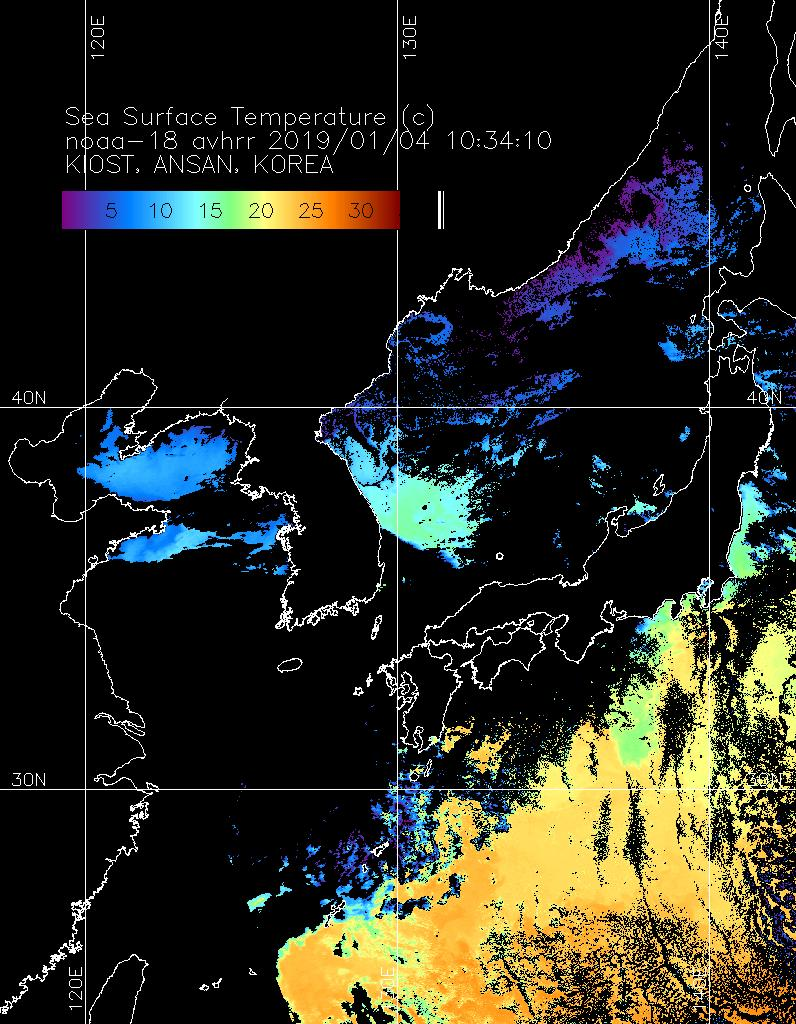
\includegraphics[width=10cm]{2019.0104.1034.noaa-18.sst}}
	\caption{KOSC에서 배포한 NOAA/AVHRR SST 자료.}
	\label{fig:SST-KOSC}
\end{figure}

KOSC로 부터 다운받아 본 연구에 사용한 NOAA/AVHRR의 SST 자료의 정보는 Table \ref{table:NOAA-data}\와 같다.

\begin{table}[!htbp]
	\caption{사용한 NOAA/AVHRR SST data.}

	\begin{tabular}{c|c|c|c|c|c}
		\hline
		
		\hline
		year   & NOAA-15 & NOAA-16 & NOAA-17 & NOAA-18 & NOAA-19 \\ 
		
		\hline
		
		\hline
		2011 & 0       & 406     & 18      & 412     & 413     \\ \hline
		2012 & 12      & 1,184   & 11      & 1,073   & 1,141   \\ \hline
		2013 & 0       & 1,229   & 0       & 1,085   & 1,145   \\ \hline
		2014 & 0       & 533     & 0       & 1,056   & 728     \\ \hline
		2015 & 0       & 0       & 0       & 1,106   & 452     \\ \hline
		2016 & 0       & 0       & 0       & 1,022   & 1,177   \\ \hline
		2017 & 0       & 0       & 0       & 818     & 1,072   \\ \hline
		2018 & 0       & 0       & 0       & 912     & 937     \\ \hline
		2019 & 0       & 0       & 0       & 847     & 843     \\ \hline
		2020 & 0       & 0       & 0       & 526     & 527     \\ 
		
		\hline

		\hline
	\end{tabular}
	\label{table:NOAA-data}
\end{table}


\newpage
\subsection{자료 처리}

NOAA/AVHRR의 SST 레벨2 자료를 위도, 경도 구간을 나눈 후, 일평균값, 주평균값, 월평균값을 산출하여 레벨3 자료를 만들었다. 자료 처리는 Phthon을 이용하여 실시하였다. 
=======
\subsection{데이터 파악 및 수집}

해양위성센터에서 제공하는 SST 데이터를 다운받을 수 있는 경로를 확인하였다. 접근할 수 있는 데이터는 2020년 4월 29일 기준으로 Table 과 같다.

2012년부터 2019년까지의 8년 동안 Terra/Aqua 위성이 MODIS를 통해 수집한 자료를 연구에 이용하기로 결정하고, Github에서 다운로드한 웹 크롤링 파일을 이용하여 해양위성센터의 SST 데이터를 크롤링하는 table 과 같이 코드를 작성하였다. 2021년 6월 현재는 천리안위성 2호가 서비스를 시작하면서 사이트가 개편되어 데이터 배포 방식이 바뀌었어 아래의 코드가 실행되지 않을 수도 있다.

온라인 원격수업 환경에서 파일을 다운로드받기 위해 Chrome Remote Desktop을 이용하여 개인 노트북을 Ubuntu 운영체제의 서버 컴퓨터와 연결하여 사용할 수 있도록 하였으며, Ubuntu 프롬프트 명령어를 사용하여 파일 디렉토리를 탐색하는 방법을 학습하였다. 오랜 시간 동안 많은 양의 데이터를 다운받아야 하기 때문에 도중에 프롬프트 창을 닫더라도 계속 다운받을 수 있도록 nohup 명령어를 이용하여 백그라운드로 파일을 실행하였다. 
>>>>>>> c2fb6d045ef38751fc9fe31d0bd3b77d1b59076f

